Segundo \citeonline{silveira2011metodologia}, metodologia consiste "em um estudo crítico e analítico dos métodos de investigação". Os métodos científicos a serem seguidos para conceber novos conhecimentos são inúmeros e compõem o estudo de estruturas de pesquisa que podem ser classificadas de acordo com sua natureza, seu objetivo, sua abordagem e seus procedimentos. \cite{nascimento2016classificaccao}. 

% Estes conceitos foram explorados anteriormente no Capítulo 1 e serão detalhados nos tópicos seguintes.

Conforme descrito por \citeonline{zanella2006metodologia}, a pesquisa apresenta diversos tipos relacionado à sua natureza, objetivos, abordagem e procedimentos. Ainda de acordo com o material, é possível dizer que a presente pesquisa possui:

\begin{itemize}

\item \textbf{Natureza:} aplicada, por ter como objetivo a solução de um problema humano;
\item \textbf{Objetivos:} exploratória, em razão de ser uma pesquisa que busca ampliar o conhecimento sobre fenômenos da comunidade acadêmica, atrás de conhecer suas necessidades e buscar tratá-las; 
\item \textbf{Abordagem:} quantitativa, visto que caracteriza-se pela ampla utilização de instrumental estatístico fundamental na análise de dados coletados;
\item \textbf{Procedimentos:} procedimento bibliográfico para investigação do referencial teórico aliado a produção tecnológica no contexto de desenvolvimento de software.

\end{itemize}

\subsection{Natureza de Pesquisa}
No que diz respeito à natureza da pesquisa, ela pode ser classificada como básica ou aplicada. Enquanto a pesquisa básica visa gerar novas verdades para a ciência, sem que aja compromisso com a aplicação prática no ambiente investigado, a pesquisa aplicada é direcionada à solução de problemas específicos \cite{nascimento2016classificaccao}. Como o projeto busca desenvolver um aplicativo com o intuito de mitigar problemas de saúde dentro de instituições acadêmicas, podemos dizer que a natureza desta pesquisa é aplicada. 

\subsection{Abordagem de Pesquisa}
Conforme também aponta \citeonline{nascimento2016classificaccao} a metodologia de pesquisa pode ser definida como uma abordagem quantitativa, qualitativa ou mista. Enquanto a abordagem quantitativa valoriza respostas estatísticas e padronizadas, o método qualitativo considera as singularidades de cada sujeito objeto da pesquisa. Ainda com base no que o autor descreve, essas abordagens, apesar de possuírem características diferentes, possuem caráter complementar e não excludente \cite{nascimento2016classificaccao}. 

Aplicado ao contexto deste trabalho, apesar de serem considerados parâmetros subjetivos para o desenvolvimento do aplicativo, ele possui como foco a utilização de ferramentas estatísticas para análise de dados coletados e consequente solução de problemas. Dessa forma, a abordagem desta pesquisa possui caráter quantitativo.

\subsection{Objetivo de Pesquisa}
Em \citeonline{silveira2011metodologia} é possível identificar a ramificação da pesquisa com base em seus objetivos em: exploratória, descritiva e explicativa. A pesquisa descritiva restringe-se a interpretar a realidade sem promover mudanças. A pesquisa explicativa busca elucidar a razão de algum fenômeno. Neste trabalho não pretende-se descrever realidades ou esclarecer porquês, portanto é considerada uma pesquisa exploratória. Esta consiste em um passo inicial de um trabalho científico que assume um caráter de pesquisa bibliográfica e estudo de caso que ajuda a formular o problema de pesquisa e seus objetivos \cite{silveira2011metodologia}. 

\subsection{Procedimento de Pesquisa}
Ainda de acordo com \citeonline{silveira2011metodologia}, os procedimentos técnicos de pesquisa incluem as categorias: bibliográfica, documental, experimental, estudo de caso, levantamento, estudo de campo, pesquisa-ação e pesquisa participante. A pesquisa bibliográfica, que é um dos procedimentos de pesquisa utilizados neste trabalho, é um procedimento efetuado a partir de material já publicado e traz a base teórica científica para o projeto. Este procedimento está presente em todas as produções acadêmicas

Adicionalmente, no contexto de desenvolvimento de software, a produção tecnológica trata-se de outro procedimento de pesquisa adotado neste trabalho que tem como objetivo o desenvolvimento de um aplicativo a fim de solucionar problemas da comunidade universitária.

\subsection{Processo Metodológico}

De acordo com a Universidade de Brasília (UnB) o Trabalho de Conclusão de Curso (TCC) deve ser dividido em duas fases, sendo elas: TCC1 e TCC2. Sendo assim, o TCC1 tem como objetivo propor um projeto viável para desenvolvimento e desenvolver a base teórica, já o TCC2 tem o objetivo de implementar o projeto proposto, de acordo com a definição realizada no TCC1.

\subsubsection{TCC1}

Dividimos o Trabalho de Conclusão de Curso 1 em etapas que podem ser vistas detalhadamente na Tabela~\ref{tab:atividades-tcc1} e na Figura~\ref{(atividades-tcc1)}.

% \begin{itemize}
%     \item Definir tema:
%     \item Definir metodologia
%     \item Realizar pesquisa bibliográfica
%     \item Elaborar proposta de solução
%     \item Realizar levantamento de requisitos
%     \item Definir arquitetura
%     \item Realizar Modelagens
%     \item Realizar Prototipação
%     \item Revisão Geral
%     \item Apresentação TCC1 
% \end{itemize}

\begin{table}[H]
    \centering
    \caption{Cronograma das Atividades do TCC1 (2025).}
    \label{tab:atividades-tcc1}

    \begin{tabular}{|l|c|c|c|c|}
    \hline
    \textbf{Atividade} & \textbf{Abr} & \textbf{Mai} & \textbf{Jun} & \textbf{Jul} \\ \hline
    Definir tema & X  &   &   &   \\ \hline
    Definir metodologia & X  &   &   &   \\ \hline
    Realizar pesquisa bibliográfica &  X & X  &   &   \\ \hline
    Elaborar proposta de solução &   & X  &   &   \\ \hline
    Realizar levantamento de requisitos &   & X  & X  &   \\ \hline
    Definir arquitetura &   &   & X &   \\ \hline
    Realizar Modelagens &   &   & X  &   \\ \hline
    Realizar Prototipação  &   &   & X  &   \\ \hline
    Revisão Geral  &   &   &   & X  \\ \hline
    Apresentação TCC1 &   &   &   & X  \\ \hline
    \end{tabular}

    \vspace{0.5em}
    \small Fonte: autoria própria.
\end{table}

\clearpage 

\begin{figure}[H]
    \centering
    \caption{Raia do TCC1 do BPMN do Processo Metodológico.}
    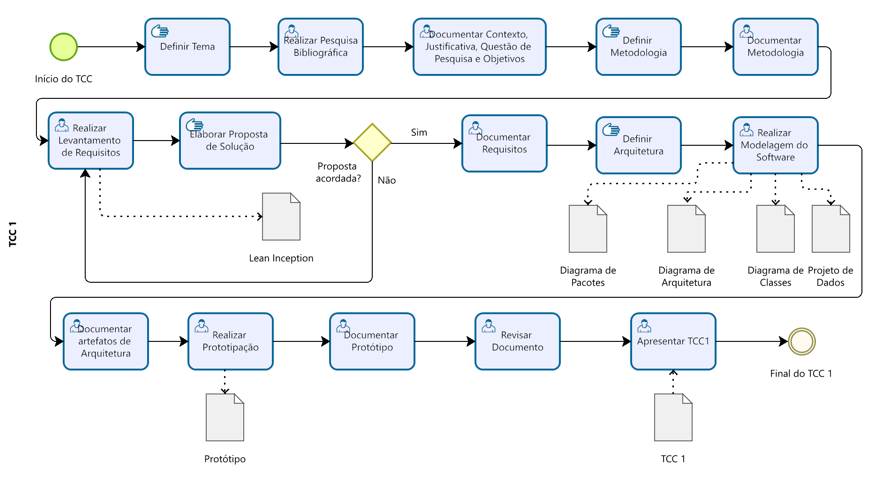
\includegraphics[width=1\textwidth]{figuras/tcc1.png}
    \par
    Fonte: autoria própria.
    \par
    \label{(atividades-tcc1)}
\end{figure}

\subsubsection{TCC2}

Além disso, delineamos também o fluxo de atividades que serão realizadas no processo de desenvolvimento do Trabalho de Conclusão de Curso 2, como pode ser visto na Figura~\ref{(atividades-tcc2)}.

\begin{figure}[H]
    \centering
    \caption{Raia do TCC2 do BPMN do Processo Metodológico.}
    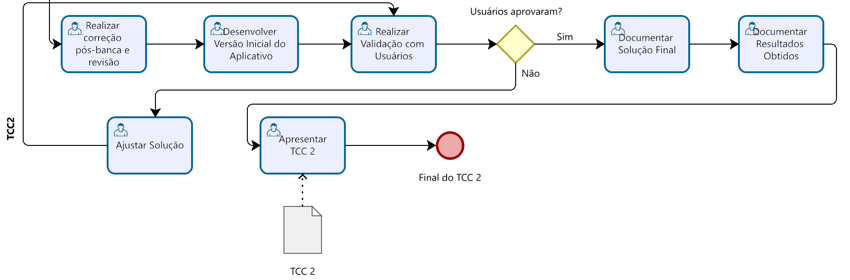
\includegraphics[width=1\textwidth]{figuras/tcc2.png}
    \par
    Fonte: autoria própria.
    \par
    \label{(atividades-tcc2)}
\end{figure}

Totalizando temos o BPMN visto na Figura~\ref{(atividades-tcc12)}.

\begin{figure}[H]
    \centering
    \caption{BPMN do Processo Metodológico}
    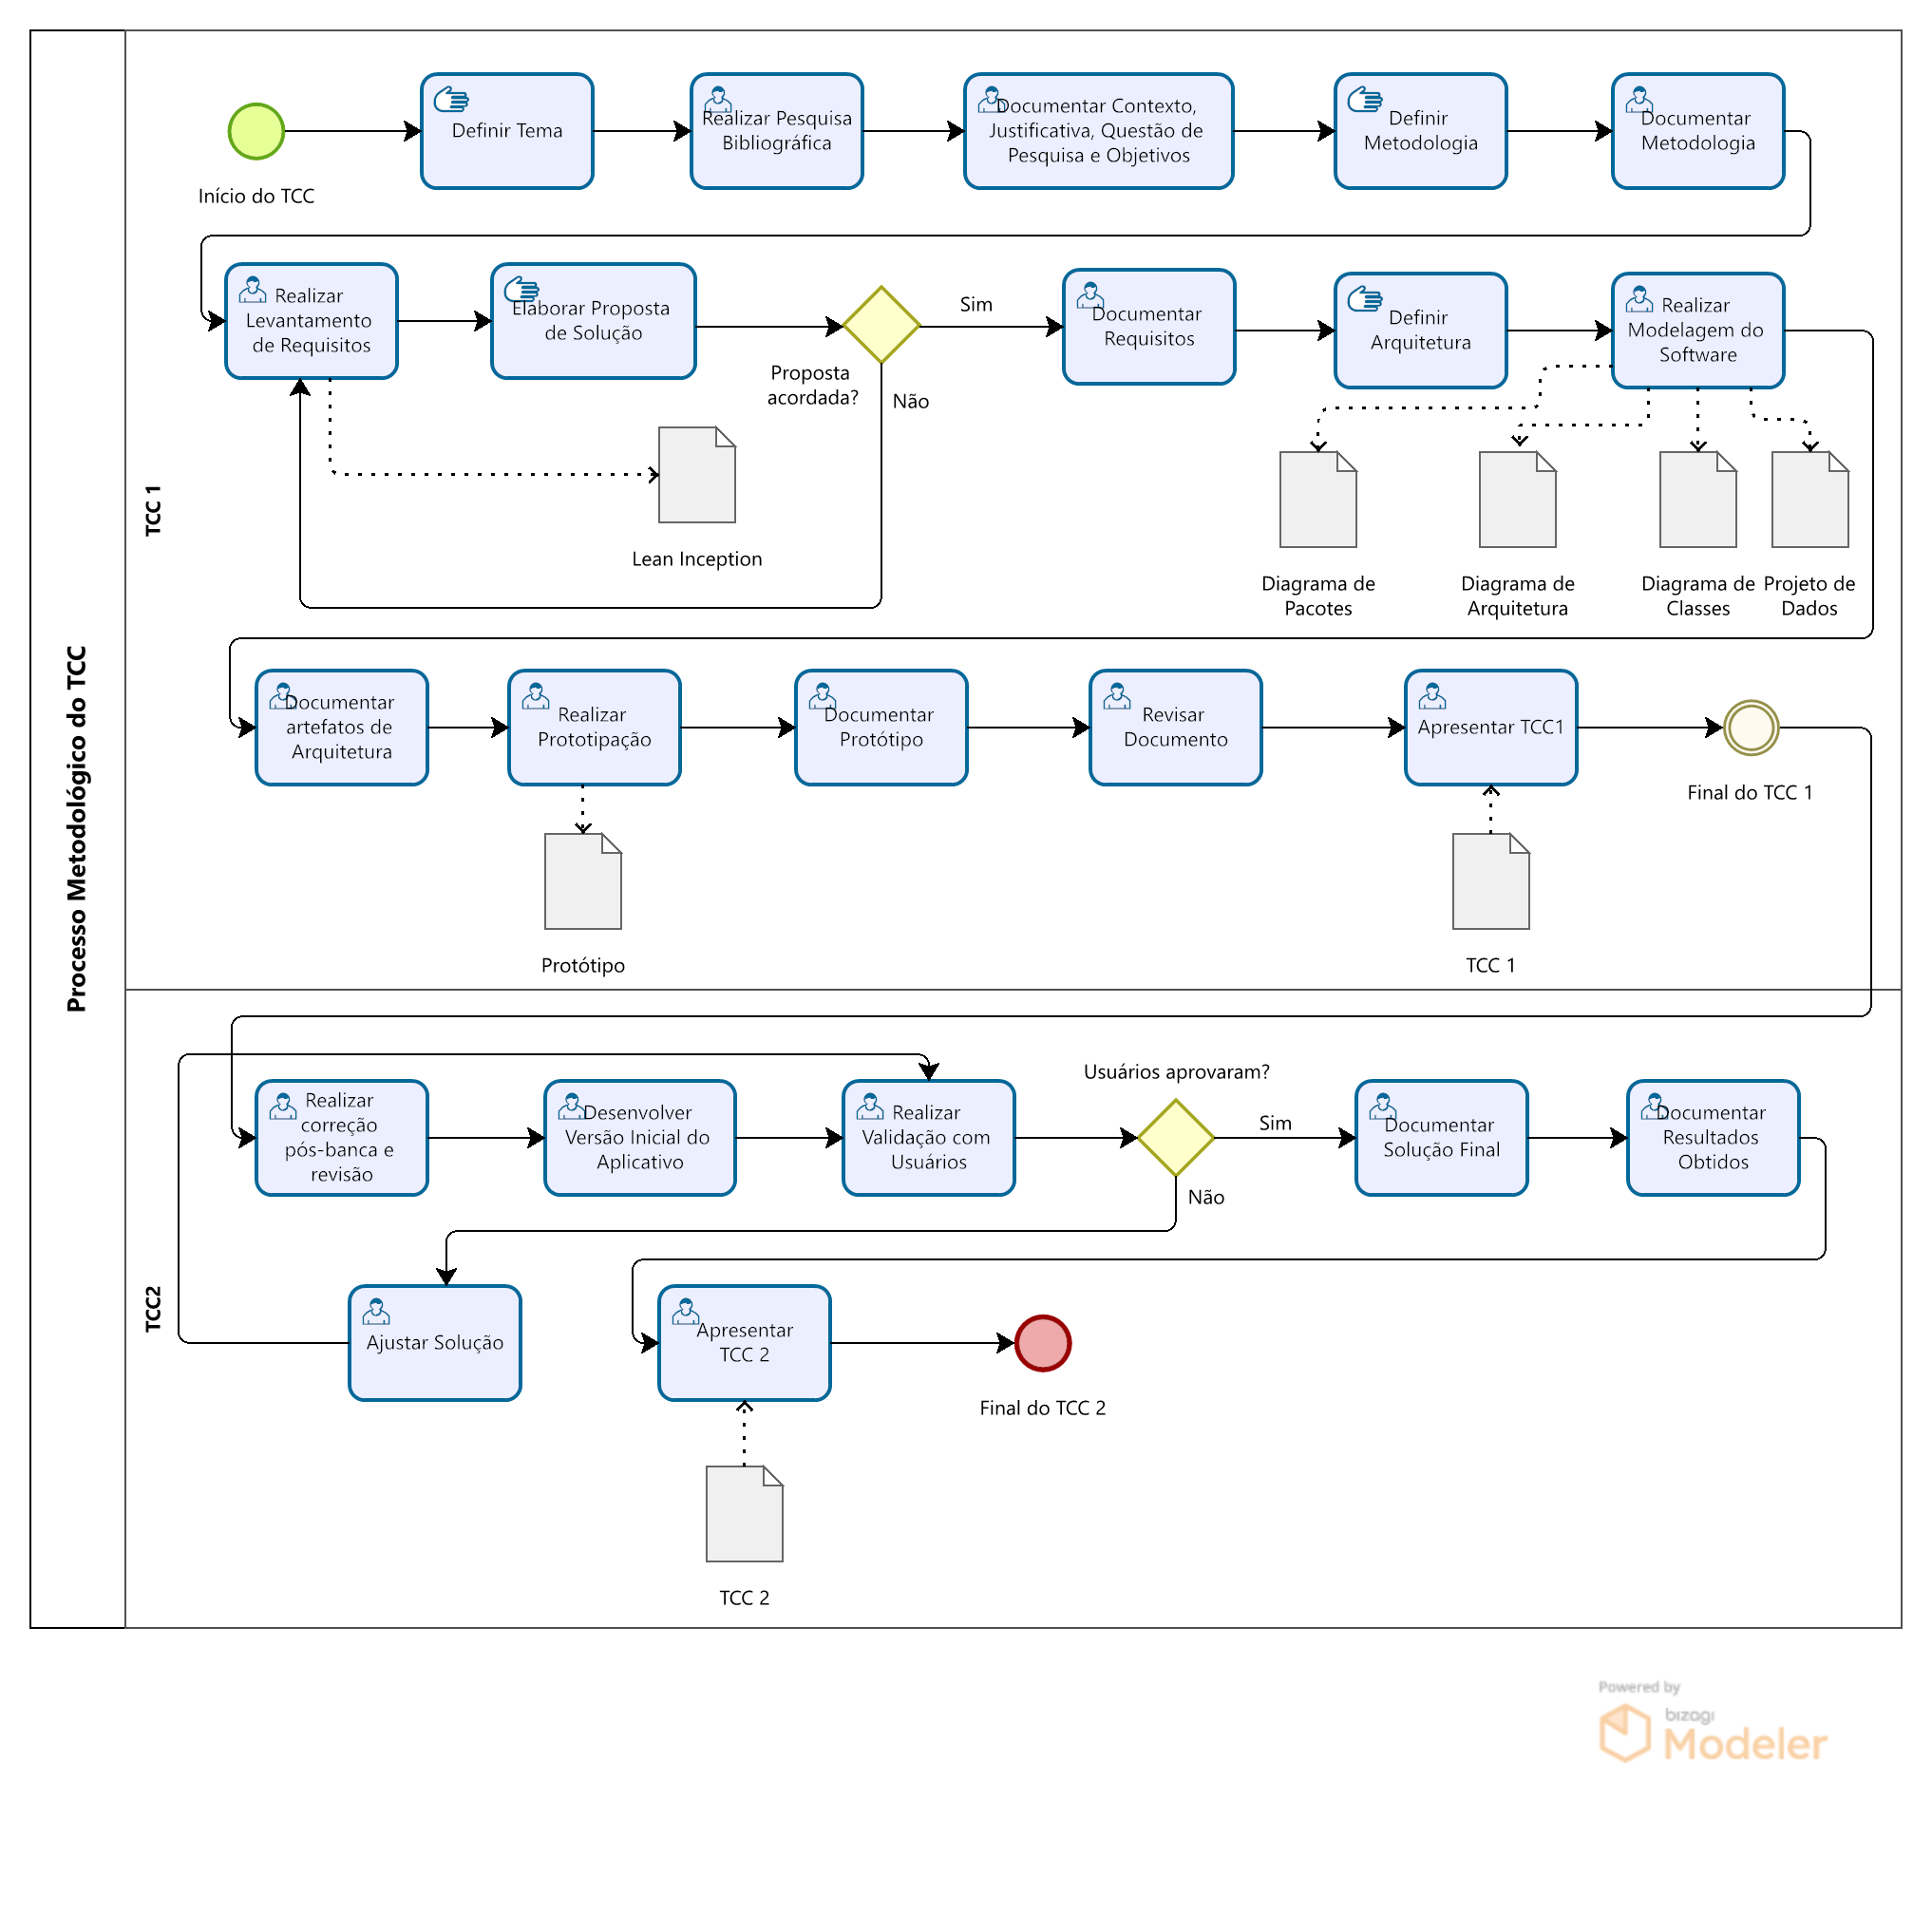
\includegraphics[width=0.9\textwidth]{figuras/bpmn_tcc12.png}
    \par
    Fonte: autoria própria.
    \par
    \label{(atividades-tcc12)}
\end{figure}

